\section*{Exercice 133 -- Schéma cinématique -- Camion benne}
\setcounter{exo}{0}
%POLE JC
On s’intéresse à un camion benne, dont une photo et un schéma cinématique sont donnés ci-dessous.


%\begin{figure}[H]
%\centering
%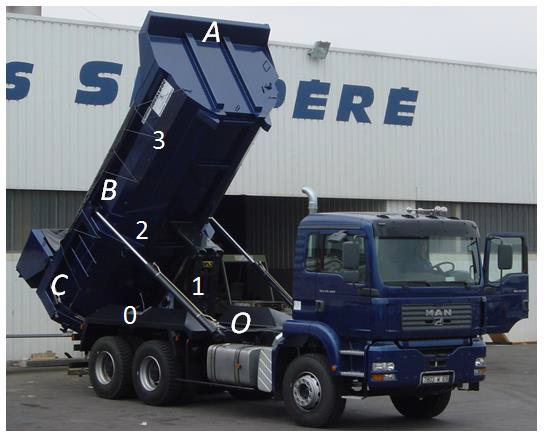
\includegraphics[width=\linewidth]{996_01}
%\end{figure}

\begin{figure}[H]
\centering
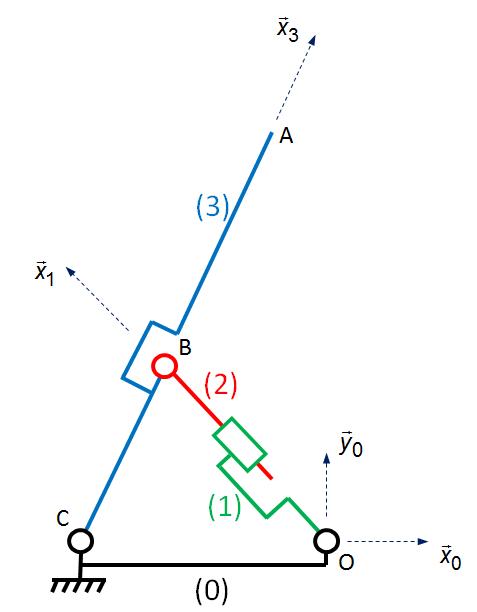
\includegraphics[width=\linewidth]{996_02}
\end{figure}

Ce système est constitué de quatre solides :
\begin{itemize}
\item le châssis 0, de repère associé  $\rep{0}\repere{O}{x_0}{y_0}{z_0}$;
\item le corps 1, d'un des deux vérins, de repère associé   $\rep{1}\repere{O}{x_1}{y_1}{z_1}$ tel que $\alpha = \angl{x_0}{x_1}$;
\item la tige 2, d'un des deux vérins, de repère associé   $\rep{2}\repere{B}{x_2}{y_2}{z_2}$ tel que $\vect{OB}=\lambda \vect{x_1}$;
\item la benne 3 de repère associé  $\rep{3}\repere{C}{x_3}{y_3}{z_3}$ tel que $\beta = \angl{x_0}{x_3}$.
\end{itemize}

Pour éviter toute collision, il est nécessaire de maîtriser parfaitement à chaque instant la position du point $A$ , fixe dans la
benne 3, par rapport au repère associé au sol.

 \begin{obj}
Appréhender le schéma cinématique en vue d’une étude géométrique ultérieure.
 \end{obj}



\subparagraph{}
\textit{Sur le schéma cinématique, repasser chaque solide d’une couleur différente. Repérer les liaisons et les lister
sur un graphe des liaisons. Préciser le paramètre de mouvement associé à chaque liaison.}
\ifprof
\begin{corrige}
\end{corrige}
\else
\fi


\subparagraph{}
\textit{Réaliser les figures de changement de base, et en déduire le vecteur vitesse angulaire associé à chacune
d’entre elles.}
\ifprof
\begin{corrige}
\end{corrige}
\else
\fi


\subparagraph{}
\textit{Que dire des bases $\mathcal{B}_1\base{x_1}{y_1}{z_1}$ et  $\mathcal{B}_2\base{x_2}{y_2}{z_2}$ ? En déduire $\vecto{2}{1}$ et $\vecto{2}{0}$.}
\ifprof
\begin{corrige}
\end{corrige}
\else
\fi
